% Please use the skeleton file you have received in the 
% invitation-to-submit email, where your data are already
% filled in. Otherwise please make sure you insert your 
% data according to the instructions in PoSauthmanual.pdf

% JRP added to avoid ifpdf name clash in TexShop
\RequirePackage{ifpdf}
%%% END JRP

\documentclass{PoS}

%JRP added
%Uncomment next line if AMS fonts required
 \usepackage{graphicx}
 \usepackage{epstopdf}

 %%% END JRP

\title{Cosmology from EoR/Cosmic Dawn}

\ShortTitle{EoR/CD Cosmology}

\author{\speaker{Pritchard}\thanks{A footnote may follow.}, Chang, Furlanetto, Choudhury, Zaroubi, Santos, Chen, Weller, Abdalla, Mesinger on behalf of the Cosmology-SWG and EoR/CD-SWG\\
        Imperial College London\\
        E-mail: \email{j.pritchard@imperial.ac.uk}}

%\author{Another Author\\
%        Affiliation\\
%        E-mail: \email{...}}

\abstract{SKA Phase 1 will build upon early detections of the EoR by precursor instruments, such as MWA, PAPER, LOFAR, and HERA, to make the first high signal-to-noise measurements of fluctuations in the 21 cm brightness temperature from both reionization and the cosmic dawn. This will allow both imaging and statistical maps of the 21cm signal at redshifts $z=6-30$ and constrain the underlying cosmology and evolution of the density field. This era includes nearly 60\% of the (in principle) observable volume of the Universe and many more linear modes than the CMB, presenting an opportunity for SKA to usher in a new level of precision cosmology. This optimistic picture is complicated by the need to understand and remove the effect of astrophysics, so that systematics rather than statistics will limit constraints.

This chapter will describe the cosmological, as opposed to astrophysical, information available to SKA Phase 1. Key areas for discussion include: cosmological parameters constraints using 21cm fluctuations as a tracer of the density field; lensing of the 21cm signal, constraints on heating via exotic physics such as decaying or annihilating dark matter; impact of fundamental physics such as non-Gaussianity or warm dark matter on the source population; and constraints on the bulk flows arising from the decoupling of baryons and photons at $z=1000$. The chapter will explore the path to separating cosmology from `gastrophysics', for example via velocity space distortions and separation in redshift. We will discuss new opportunities for extracting cosmology made possible by the sensitivity of SKA-1 and explore the advances achievable with SKA-2.
}

\FullConference{
Advancing Astrophysics with the Square Kilometre Array\\
June 8-13, 2014\\
Giardini Naxos, Italy}

%Add new definitions here
%user defined shortcuts
%Journal definitions
\newcommand{\apj}{ApJ}
\newcommand{\apjl}{ApJ}
\newcommand{\apjs}{ApJS}
\newcommand{\aap}{A \& A}
\newcommand{\aj}{AJ}
\newcommand{\araa}{ARAA}
\newcommand{\mnras}{MNRAS}
\newcommand{\physrep}{Phys. Rep.}
\newcommand{\prd}{PRD}
\newcommand{\nat}{Nat.}
\newcommand{\jcap}{JCAP}
\newcommand{\sovast}{Sov. Astron.}
\newcommand{\nar}{New Astron. Rev.}
\newcommand{\apss}{Astrophys. \& Space. Sci.}

\newcommand{\ud}{{\rm d}}

%%%% END NEW DEFINITIONS

\begin{document}

%%%%%%%%%%%%%%%%%%%%%%%%%%%%%
%%%%%%%%%%%%%%%%%%%%%%%%%%%%%
\section{Introduction}

The years since the COBE observations of the CMB have ushered in an age of precision cosmology. Key cosmological parameters have been made possible by measurements of the distribution of matter in the Universe through WMAP and Planck observations of CMB anisotropies and large volume galaxy surveys such as SDSS. These surveys have made precision measurements of parameters describing the matter content of the Universe - the baryons $\Omega_b$, dark matter $\Omega_c$, dark energy $\Omega_\Lambda$, radiation $\Omega_r$, and neutrinos $\Omega_\nu$ - and the physics of inflation - via the tilt $n_s$, amplitude $A_s$, running $\ud n_s/\ud\log k$ or the primordial potential power spectrum and $r$ the ratio of tensor-to-scalar modes produced by inflation. These measurements have firmly established the basic picture of our Universe, known widely as the $\Lambda$CDM model of cosmology.

Despite this progress, measuring these numbers is only the first step towards a deep understanding of the underlying physics. Our ignorance of the nature of the dark matter and the dark energy or how neutrinos acquire mass and what value that mass takes are just two questions that modern cosmology hopes to address. Over the next decade two paths will help shed light on this. The simplest is simply to measure these cosmological parameters ever more precisely and over a wider range of times and scales in the hope of gaining further insights. The exemplar of this is with dark energy, where attempts to measure the redshift evolution of the dark energy density, parameterised by an equation of state $w(z)$, might distinguish a true cosmological constant from more general dark energy or modified gravity. For others there are critical thresholds of precision required to distinguish physical scenarios - for example, measuring the sum of the neutrino masses $M_\nu\lesssim0.1$ would determine the neutrino mass hierarchy. Clearly more precision is a good thing, but it is not the only path forward.

Secondly, we can seek signatures of new physics in ways distinct from the distribution of large scale matter. The processes that produce dark matter will also allow it to annihilate and maybe to decay. The release of energy might have impact on the surrounding environment, heating the intergalactic medium. Pursuing unique signatures of new physics in new regimes will be a key part of the next decade.

The SKA is uniquely placed to probe cosmology as it is capable of mapping the Universe over wide volumes and an unprecedented range of redshifts. Figure \ref{fig:volume} illustrates the additional range of volume and redshifts that the SKA will constrain. In this chapter, we will focus on the new opportunities created by SKA observations of the epoch of reionization (EoR) and the cosmic dawn (CD). This period has never before been observed offering a unique opportunity to test the consistency of the $\Lambda$CDM model and search for new hints to the great unanswered questions of cosmology.

\begin{figure}[htbp]
\begin{center}
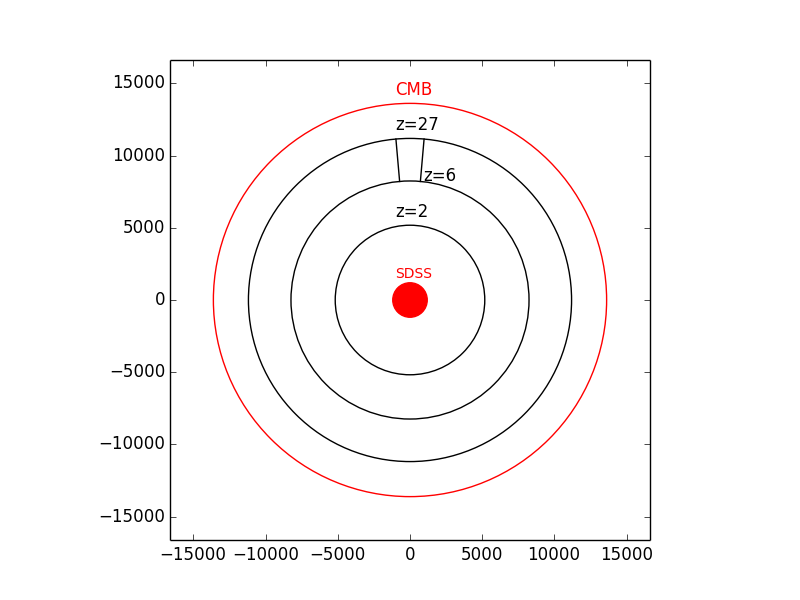
\includegraphics[scale=0.6]{figures/plotcircles.png}
\caption{Illustration of the volume probed by SKA}
\label{fig:volume}
\end{center}
\end{figure}

\cite{furlanetto2006dm}

\begin{figure}[htbp]
\begin{center}
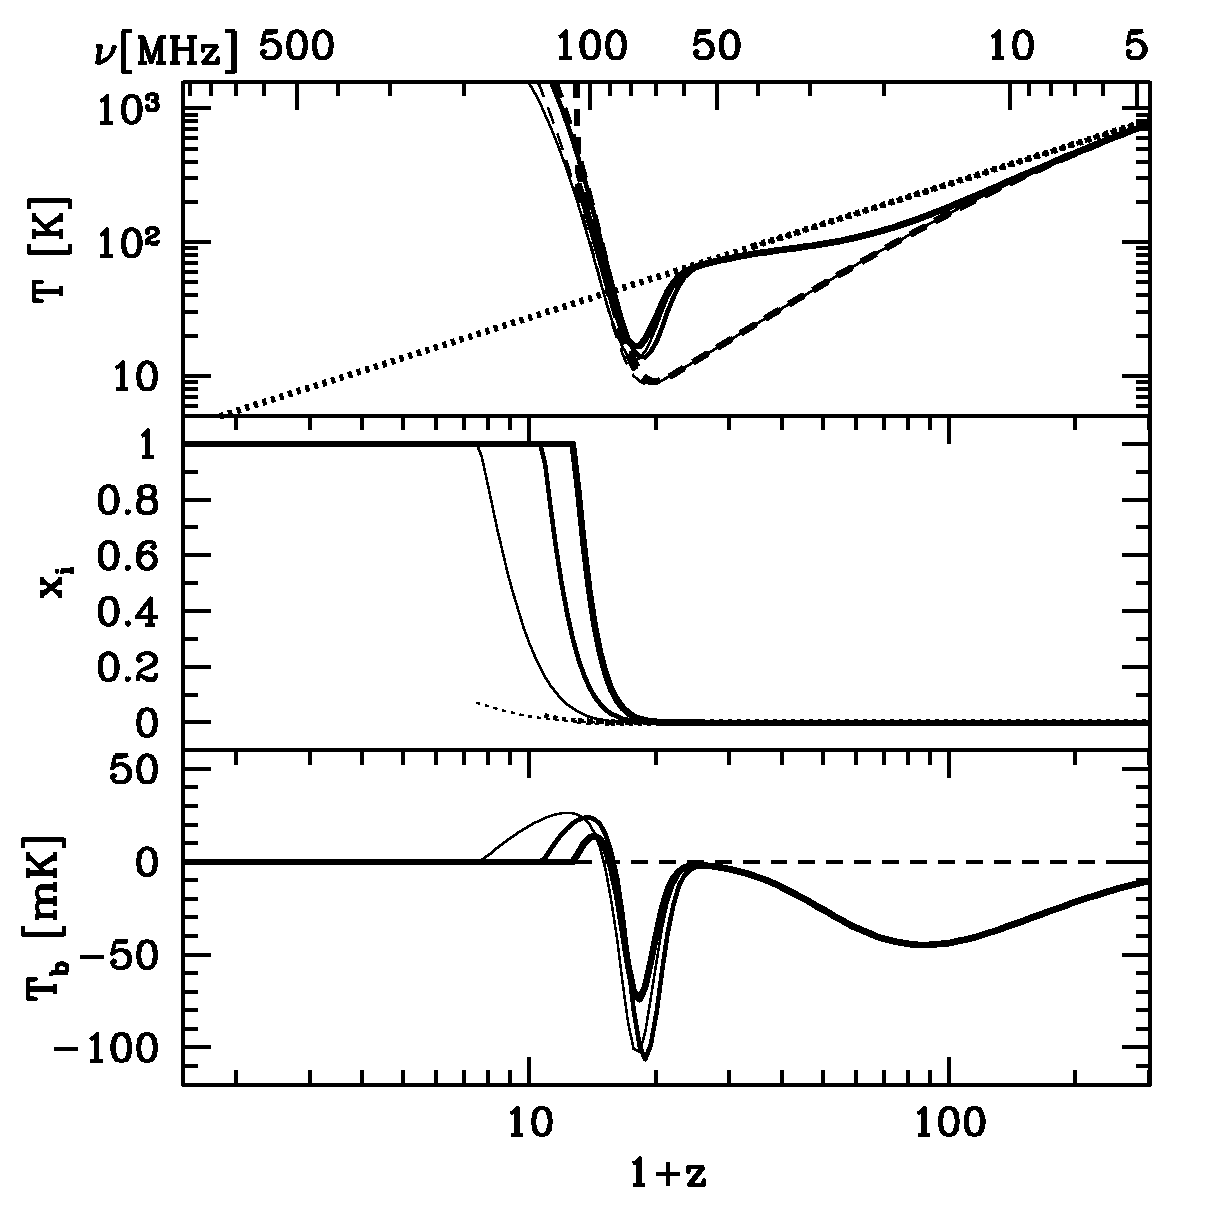
\includegraphics[scale=0.3]{figures/global_signal.eps}
\caption{This is a test figure}
\label{fig:global_signal}
\end{center}
\end{figure}

{\bf Introductory chapter}


%%%%%%%%%%%%%%%%%%%%%%%%%%%%%
%%%%%%%%%%%%%%%%%%%%%%%%%%%%%
\section{Cosmological parameters from density fluctuations}

{\bf Introduce fisher matrix formalism}

{\bf sensitivity plot for various experiments relative to density field}

{\bf concept of effective volume and how SKA compares to various galaxy surveys}

\begin{figure}[htbp]
\begin{center}

\caption{Sensitivity plots of SKA1 (30\%), SKA1 (full), and SKA2}
\label{fig:sensitivity}
\end{center}
\end{figure}

\subsection{Core cosmological parameters}

\subsection{Inflationary parameters}

\subsection{Neutrino mass}



%%%%%%%%%%%%%%%%%%%%%%%%%%%%%
%%%%%%%%%%%%%%%%%%%%%%%%%%%%%
\section{Constraining new physics from heating}

%%%%%%%%%%%%%%%%%%%%%%%%%%%%%
%%%%%%%%%%%%%%%%%%%%%%%%%%%%%
\section{Fundamental physics from modifications to the source population}

%%%%%%%%%%%%%%%%%%%%%%%%%%%%%
%%%%%%%%%%%%%%%%%%%%%%%%%%%%%
\section{Bulk flows}

%%%%%%%%%%%%%%%%%%%%%%%%%%%%%
%%%%%%%%%%%%%%%%%%%%%%%%%%%%%
\section{Cosmic shear and the EoR}

Ben Metcalf to prepare a summary updated for SKA parameters.

%%%%%%%%%%%%%%%%%%%%%%%%%%%%%
%%%%%%%%%%%%%%%%%%%%%%%%%%%%%
\section{Separating ``gastrophysics" and cosmology}

%%%%%%%%%%%%%%%%%%%%%%%%%%%%%
%%%%%%%%%%%%%%%%%%%%%%%%%%%%%
\section{Paths to cosmology with Phase 1 and Phase 2}

%%%%%%%%%%%%%%%%%%%%%%%%%%%%%
%%%%%%%%%%%%%%%%%%%%%%%%%%%%%
\section{Miscellaneous?}

%%%%%%%%%%%%%%%%%%%%%%%%%%%%%
%%%%%%%%%%%%%%%%%%%%%%%%%%%%%

%JRP use bibtex while editing
\bibliographystyle{unsrt}
\bibliography{cosmchapterbib}{}
%%% END JRP

%%% Fill copy in .bbl at end
%\begin{thebibliography}{99}
%\bibitem{...}
%\end{thebibliography}
% END COMMENTED OUT BIB

\end{document}
